\documentclass[12pt,a4paper,ngerman]{scrartcl}

\usepackage[ngerman]{babel}
\usepackage[utf8]{inputenc}
\usepackage[T1]{fontenc}
\usepackage{csquotes}
\usepackage{graphicx}


\author{Thomas Hilarius Meyer\\ \textsf{thomas.hilarius.meyer@gmail.com}}
\title{Die Gersheimer Schulimkerei-Beute (GeSIB)}
\subtitle{Überlegungen zu Konzeption, Bau und Betriebsweise}


\begin{document}
	\maketitle

        
\begin{abstract}
	Die Gersheimer Schulimkerei-Beute (GeSIB) ist eine Trogbeute für 24 Waben im Zander-Maß.
	Sie eignet sich besonders für den pädagogisch motivierten Umgang mit Bienen, da alle Waben in einer
	Ebene liegen und somit direkt einsehbar und zugänglich sind; im Umgang mit ihr sind
	keine schweren Gewichte zu heben und die Arbeitshöhe bleibt konstant.
	Alle Verfahren der modernen Magazin-Imkerei lassen sich mit der GeSIB durchführen und
	ein späterer Wechsel der Jungimker etwa zu üblichen Magazinbeuten ist problemlos möglich.
\end{abstract}


\section{Gestaltungsprinzipien}

Die Zeit ist reif für einen neuen Bienenkasten, der speziell auf die Bedürfnisse einer Schulimkerei und ihrer Mitglieder --
besonders in den ersten 1--2 Jahren des Imkern-Lernens -- ausgelegt ist!

Die Mitglieder der Schulimkerei Gersheim haben eine Bienenbeute entwickelt, die sich ausschließlich diesem Ziel widmet:
die Gersheimer Schulimkerei-Beute (GeSIB).

Nach einem angemessenen Erprobungsbetrieb könnte die Herstellung der GeSIB die Angebotspalette unserer Schüllerfirma
entscheidend erweitern.


\subsection{Vorüberlegungen / Anforderungen}

Was müsste ein Schulbienenkasten besser können als die Liebig-Beute?

\begin{enumerate}
\item Die Imkerneulinge sollen keine Zargen abheben müssen, denn dies bedeutet...
  \begin{itemize}
  \item eine Frage der Kraft,
  \item ist eine psychologische Hemmschwelle
  \item  und eine Störung der Bienen.
  \end{itemize}
\item Alle Teile des Bienenstocks sollen gleichzeitig sichtbar sein (von oben, auf einen Blick),
\item das Wabenmaß soll das weit verbreitete Zandermaß sein,
  um später leichter auf Magazinbeuten umsteigen zu können (eine Beute, aus der man \enquote{herauswächst}...),
\item die Betriebsweise soll sehr nahe an der Magazinimkerei liegen (imkern lernen) und
\item der Bau soll zu einem geringen Preis und
\item mit wenig Aufwand möglich sein.
\end{enumerate}

In Kauf genommene Nachteile sind weitgehend irrelevant für den speziellen Zweck der \enquote{pädagogischen} Bienenbeute:

\begin{itemize}
\item \enquote{Unwirtschaftliches} Arbeiten (\enquote{wabenweise} statt \enquote{zargenweise}) -- es geht nicht um Erwerbsbienenhaltung,
  sondern um pädagogisch orientiertes Imkern.
\item Schwieriges Wandern wegen des hohen Beuten-Gewichts -- eine Schulimkerei ist erfahrungsgemäß immer eine Standimkerei.
\end{itemize}


\subsection{Konkrete Designentscheidungen}

Folgende Konstruktionsentscheidungen sind für den Entwurf maßgeblich:

\begin{itemize}
\item Zander-Rähmchen als verbreitetstes Rähmchenmaß,
\item gleiches Maß im Brut- und Honigraum,
\item Möglichkeit eines vertikalen Königinnenabsperrgitters und
\item einer vertikalen Bienenflucht,
\item extrem leichter Zusammenbau aus wenigen, einfachen Teilen.
\end{itemize}


\section{Bisherige Ansätze}

Welche Bienenkästen mit grundsätzlich ähnlicher Konstruktion (Waben auf einer Ebene) gibt es schon und warum sind diese
für die speziellen Zwecke einer Schulimkerei nicht oder nicht optimal geeignet?

\begin{description}
\item[Hohenheimer Einfachbeute] ideales System für \enquote{erwachsene} Imker; doch Nachteil: schweres Heben, Scheu des Zargen-Abhebens...
\item[Golzbeute] komplizierter Aufbau, teuer, spezielles Wabenmaß (Kuntzsch hoch), keine Bienenflucht.
\item[Mellifera Einraumbeute] spezielles Wabenmaß, kein Abspergitter und keine Bienenflucht möglich.
\item[Top-Bar-Hive] Umstieg auf Magazin-Imkerei sehr kompliziert.
\item[Bienenkiste] extrem unergonomisch; Stabilbau verhindert Wabenkontrolle.
\item[Kunesa-Beute] extrem hoher Preis; Werkstoff Kunststoff erlaubt kein handwerkliches Arbeiten (Reparaturen etc.).
\item[BienenBox] Format Kuntzsch (hoch)  (www.bienenbox.de)
\item[Citybox (Fa. Holtermann)] hoher Preis, teilweise überspezielle Features
\item[Alpentrogbeute (V. Weber)] komplizierter Aufbau, schwer zu bekommen, Honigräume werden aufgesetzt!
\end{description}


\section{Bau}

\minisec{Planskizze}

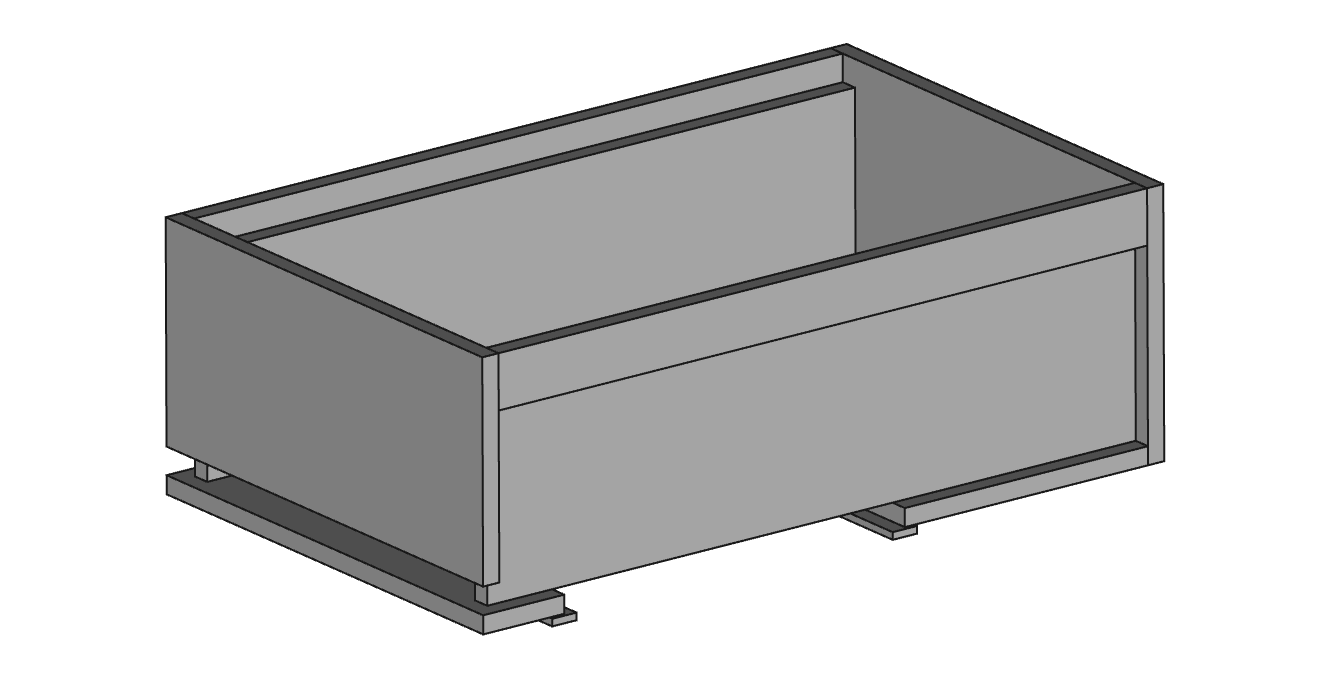
\includegraphics[width=\textwidth]{ansicht1}

\begin{center}
  [vgl. separate FreeCAD-Datei bzw. PDF-Pläne für konstruktive Details.]
\end{center}


\minisec{Teileliste}

\begin{center}
\begin{tabular}{lll}
  Bezeichnung &                       Maße [in mm] &          Anzahl \\
  \hline
  Seitenbrett links + rechts &        800 x 240 &             2 \\
  Seitl. Griffbrett links + rechts &  800 x 60 &              2 \\
  Stirnbrett vorne &                  540 x 245 &             1 \\
  Rückwand &                          540 x 290 &             1 \\
  Bodenbrett hinten &                 540 x 300 &             1 \\
  Bodenbrett vorne &                  540 x 100 &             1 \\
  Schubleisten &                      540 x 30 x 8 &          2 \\
  \hline
  Innendeckel (Dämmmaterial) &        850 x 540 &             1 \\
  \hline
\end{tabular}

[Materialstärke 25mm wenn nicht angegeben.]
\end{center}


\minisec{Zusatzteile}

\begin{center}
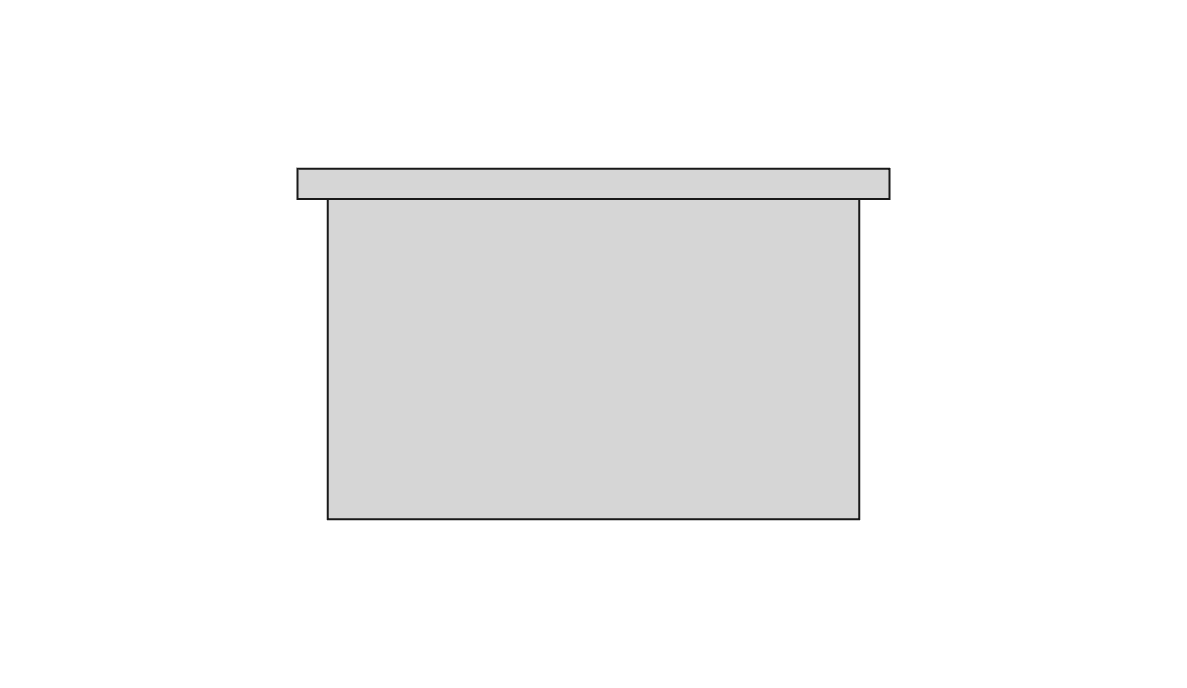
\includegraphics[width=.5\textwidth]{schiet}

\begin{tabular}{ll}
  Bezeichnung &                       Maße [in mm] \\
  \hline
  Trägerleiste &                      490 x 25 x 10 \\
  Schiet-Brett &                      440 x 265 x 10 \\
  \hline
\end{tabular}
\end{center}


Zum Betrieb werden drei Varianten eines vertikalen Trennschieds benötigt:

\begin{itemize}
\item das Trennschied selbst, um v.\,a. im Winter den Innenraum der Beute zu begrenzen,
\item ein vertikales Königinnenabsperrgitter und 
\item eine vertikale Bienenflucht.
\end{itemize}


\section{Offene Fragen}

Folgende Punkte sollen während des ersten Jahres Erprobungsbetrieb untersucht werden, um ggf. die Konstruktion noch zu verändern:

\begin{enumerate}
%\item Boden: Öffnungen wegen Belüftung und besserer Varroabeobachtung? Oder reicht die Zugänglichkeit über das Flugloch?
%  (Stabilität der Konstruktion)
\item Notwendigkeit des Abspergitters: evtl. unnötig wg. des natürlichen Triebs der Königin, das Brutnest fluglochnah zusammenzuhalten?
\item Effektivität der vertikalen Bienenflucht?
\end{enumerate}


\section{Betriebsweise}

Die imkerliche Betriebsweise mit der GSIB ähnelt grundsätzlich sehr stark den Verfahrensweisen in der Magazin-Imkerei (Liebig 2011):


\subsection{Varroa: Winterbehandlung mit Oxalsäure}

Die Bekämpfung der Varroamilbe im brutfreien Zustand im Winter kann problemlos sowohl durch Träufeln von oben als auch durch Verdampfen von unten erfolgen.
Durch die flache Bauweise wird der Bienensitz nur minimal gestört.

%(Idee: Einblasloch im Fluglochstück? Entwicklung eines Verdampfers auf Basis eines Gasbrenners?)


\subsection{Ablegerbildung}

Die Vermehrung der Völkerzahl durch die Bildung von Ablegern erfolgt 
entweder durch Bildung in der GeSIB (mit Fluglochverkleinerung und Volumenbegrenzungsschied)
oder in normalem Zander-Ablegerkasten (gleiches Wabenmaß).


\subsection{Honigernte}

Durch die Benutzung des vertikalen Absperrgitters sowie 
der vertikale Bienenflucht
gestaltet sich die Honigernte einfach und ohne massiv mit den Bienen in Kontakt zu kommen.


\subsection{Varroa: Sommerbehandlung mit Ameisensäure}

Die Sommerbehandlung der Varroamilbe erfolgt am einfachsten durch Einsatz der bekannten
Nassenheider Professional-Verdunster im bisherigen Honigraum.


\subsection{Einfütterung}

Der Futtereimer findet ebenfalls problemlos im Honigraum Platz.


\subsection{Überwinterung}

Zur Erhaltung des Stockklimas ist der Einsatz des Trennschiedes während des Winters notwendig, das eng an die besetzten Waben herangerückt wird.
Die thermischen Eigenschaften der GeSIB sind dann nicht ungünstiger als bei einer Magazinbeute.


\section{Chronologie}

\begin{description}
\item[Herbst 2017] erste Vorüberlegungen
\item[Januar/Februar 2018] Planskizze
\item[Imkersaison 2018] Erprobungsbetrieb in Gersheim
\end{description}


\section{Literaturhinweise}

\begin{enumerate}
\item Gerhard Liebig, Einfach imkern, (3. Aufl.) 2011.
\item Friedrich Pohl (Hg.), Bienenkiste, Korb und Einfachbeuten. Naturnah und erfolgreich imkern, Stuttgart 2013.
\item Johannes Weber, Bienen halten mit der BienenBox, Stuttgart 2016.
\item Vinzenz Weber, Leichter imkern mit Trogbeuten, München (2. Aufl.) 1990.
\end{enumerate}
\end{document}